\documentclass{article}

\usepackage{pgf}
\usepackage{tikz}
\usetikzlibrary{arrows}
\usepackage{subfigure}

\begin{document}
\title{An Atlas of discrete morphogenetic regulatory networks}
\maketitle

\begin{flushleft}

\section{Initial formulation of the problem}

\subsection{Open questions and degress of freedom}

\begin{enumerate}
  \item How to set the maximum thresholds of the network: in the Thomas
  framework, the maximum threshold is given by the number of outgoing edges, but
  one could introduce multiple edges in order to increase the impact of a
  predecessor on a successor node. This question might be investigated
  systematically.
  \item How to set the edge labels of the network: e.g. is an activating node
  {\tt +} or just {\tt obs+} or even another edge label? Again, this question
  might be investigated systematically.
  \item How to exactly define a stripe? This question must be investigated
  systematically, both in terms of CTL and in terms of AL.
  \item Furthermore, the intersection of the CTL and AL parameter sets must be
  investigated. Are the same parameter sets filtered by AL and CTL? I.e., is a
  stripe under CTL the same as a stripe in AL? If not, is one approach more
  comprehensive than the other?
\end{enumerate}

Note: for the stripe, we need at least three different values for the morphogene
(high, medium, low). Hence we need to artificially introduce those---either by
multi-edges or by more than one formal morphogene. E.g. two formal, identical
morphogenes are able to produce three different states of activity: both
inactive (low), one active (medium), both active (high).

\subsection{Outline of the research program}

\begin{enumerate}
  \item We will investigate one particular network with only 3 nodes (4 or 5
  with morphogene).
  \item We will apply the strictest possible edge labels ({\tt +} and {\tt -}
  initially).
  \item The dynamics are to be investigated in particular using Cytoscape.
  \item We will try out all possible values for thresholds and record the
  results for each set.
  \item Results are to be recorded for CTL filtering, for AL filtering and for
  the combination of CTL filtering and AL filtering.
  \item Next the edge label strictness can be relaxed. Again, all results are to
  be recorded.
  \item Afterwards, this procedure is to be applied for all simple
  stripe-generating networks with three nodes (diffusion to be left out initially).
  \item Finally, networks with more nodes can be investigated.
\end{enumerate}

\subsection{Other To Dos}

\begin{enumerate}
  \item Describe the connection between the quasi-continous formalism and the
  Thomas formalism
  \item Enumerate all possible (connected) networks in Python
\end{enumerate}

\begin{figure}
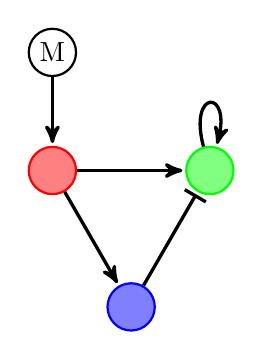
\begin{tikzpicture}
[->,>=stealth',shorten >=1pt,
gene/.style={circle,thick,inner sep=0pt,minimum size=6mm}]
\node[gene,draw=black,fill=white]    at (90:1.5cm)  (mm) {M};
\node[gene,draw=red,fill=red!50]     at (0,0)     (rr) {};
\node[gene,draw=blue,fill=blue!50]   at (300:2cm) (bb) {};
\node[gene,draw=green,fill=green!50] at (0:2cm)   (gg) {};

\path [->,very thick] (mm) edge node {} (rr);
\path [->,very thick] (rr) edge node {} (gg);
\path [->,very thick] (rr) edge node {} (bb);
\path [-|,very thick] (bb) edge node {} (gg);
\path [->,very thick] (gg) edge [loop above,looseness=12] node {} (gg);
\end{tikzpicture}
\end{figure}

\section{Defining stripes}

\subsection{Defining stripes in CTL}

The aim of this section is to define what is meant by a ``stripe'' in the
Thomas framework as it is instantiated in the SWP tool. % FIXME: name of tool?
To this end, it is to be noted that in the SWP tool, CTL (and PCTL) formulas can
be filtered by the model checker in two different modes, {\tt forAll} (the default mode) and
{\tt exists}. To understand the difference between these modes, we consider how
a STG is mapped to a computation tree which is processed by the model
checker. An example is displayed in Fig.~\ref{STG2CT}.

\begin{figure}[h!]
\centering 
\subfigure[A (non-unitary) state transition graph] {
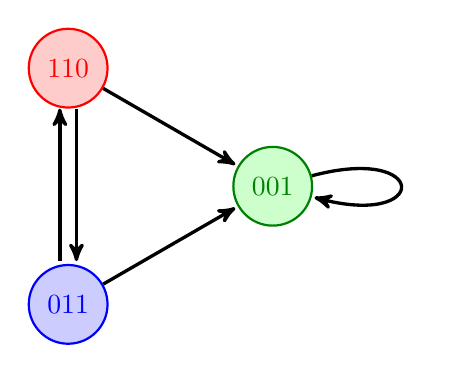
\begin{tikzpicture}
[->,>=stealth',shorten >=1pt,
gene/.style={circle,thick,inner sep=0pt,minimum size=10mm}] 
\node[gene,draw=red,fill=red!20]     at (0,0)     (rr) {\color{red}110};
\node[gene,draw=blue,fill=blue!20]   at (270:3cm) (bb) {\color{blue}011}; 
\node[gene,draw=green!50!black,fill=green!20] at (330:3cm) (gg) {\color{green!50!black}001};

\path [->,very thick] (rr) edge node {} (gg);
\draw [->,very thick] ([xshift= 3pt] rr.south) -- ([xshift= 3pt] bb.north);
\draw [<-,very thick] ([xshift=-3pt] rr.south) -- ([xshift=-3pt] bb.north);
\path [->,very thick] (bb) edge node {} (gg);
\path [->,very thick] (gg) edge [loop right,looseness=15] node {} (gg);
\end{tikzpicture}
}\hfill
\subfigure[One out of three corresponding computation trees]
{
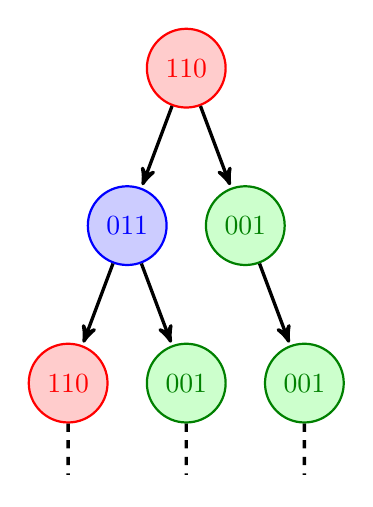
\begin{tikzpicture}
[->,>=stealth',shorten >=1pt,
gene/.style={circle,thick,inner sep=0pt,minimum size=10mm}] 
\node[gene,draw=red,fill=red!20]{\color{red}110}[level distance=20mm]
	child [->,very thick]{node [gene,draw=blue,fill=blue!20]{\color{blue}011}
		child [->,very thick]{node [gene,draw=red,fill=red!20]{\color{red}110}
			[level distance=12mm]child [-,dashed,very thick]
		}
		child [->,very thick]{node [gene,draw=green!50!black,fill=green!20]{\color{green!50!black}001}
			[level distance=12mm]child [-,dashed,very thick]
		}
	}
	child [->,very thick]{node [gene,draw=green!50!black,fill=green!20]{\color{green!50!black}001} 
		child[missing]
		child [->,very thick]{node [gene,draw=green!50!black,fill=green!20]{\color{green!50!black}001}
			[level distance=12mm]child [-,dashed,very thick]
		}
	};
\end{tikzpicture}}
\caption{Mapping from the state transition graph to a computation tree}
\label{STG2CT}
\end{figure}

We note that in order to convert an STG to a computation tree, the STG must be
rooted as well as ``expanded''. There are equally many ways to root the STG as
there are nodes in the STG. What the function {\tt filter\_byCTL(formula, mode)}
does is, given a CTL formula $\varphi$, 
\begin{itemize}
  \item if {\tt mode == 'forAll'}: it rejects all parameter sets for which
  $\varphi$ evaluates to {\tt False} no matter which state in the STG is used to
  root the computation tree,
  \item if {\tt mode == 'exists'}: it rejects all parameter sets for which
  $\varphi$ evaluates to {\tt False} in at least one computation tree
  corresponding to the STG (i.e. for at least one choice of root).
\end{itemize}

Assuming a non-empty STG, the {\tt forAll} mode is stricter than the {\tt
exists} mode.

It should be noted that in the {\tt exists} mode, there is no way to determine
the starting state (the root) of the computation tree. However, in a dynamical
problem like morphogenesis, one would like to control the starting state or
initial condition of the system. To accomplish this, we use the following
construction: we work in the stricter {\tt forAll} mode and filter by CTL
formulas of the structure
\begin{equation}
{\tt initial\_condition -> final\_condition}.
\end{equation}

On the structure of final condition and biological interpretation\ldots

\subsection{Defining stripes in AL}

in AL

\subsection{The Database}

\subsubsection{Database structure}

\begin{figure}[h!]
\centering 
\includegraphics[width=10cm]{ERDiagramRegNetTool.png}
\end{figure}

Check: are diagram and implementation consistent???

\subsubsection{Encoding and Decoding Contexts and Parameter Sets}

\end{flushleft}
\end{document}
